\documentclass[unknownkeysallowed, 10pt, a4 paper, handout]{beamer}

% Custom beamer theme
\usepackage{../style/beamerthemeCustom}
\newcommand{\HRule}{\rule{\linewidth}{0.5mm}}   %FOR TITLEPAGE

\usepackage{changepage}       % adjustwidth
\usepackage{upquote}

\setlength\parskip{0.3cm}

\newcommand{\focus}[1]{\textbf{\textcolor{red}{#1}}}
\newcommand{\expire}[1]{\textbf{\textcolor{green}{#1}}}
\newcommand{\ra}{$\longrightarrow$ }
\newcommand{\lra}{$\longleftrightarrow$ }

\newcommand{\code}[1]{\colorbox{black}{\color{green}\texttt{#1}}}

% Command to create two side-by-side minipages
\newcommand{\sidebyside}[5]{
  \begin{minipage}{#1\textwidth}
    #2
  \end{minipage} #3 \begin{minipage}{#4\textwidth}
    #5
  \end{minipage}
}

\title[Linux Programming]{ICTP DP Linux Basic Course - Programming}
\subtitle{ESP Students - First Semester}
\author[Graziano Giuliani]{Graziano Giuliani \\ \focus{ggiulian@ictp.it}}
\institute[ICTP]{The Abdus Salam International Centre for Theoretical Physics}
\date[\today]{ICTP Diploma Program \\ \today}

\begin{document}

\begin{frame}
  \titlepage
\end{frame}


\begin{frame}[label=outline]
  \frametitle{Course Outline \footnotemark}
  \framesubtitle{Daily program}
  \begin{itemize}
    \item \expire{UNIX/Linux}
    \item \focus{Programming on Linux}
      \begin{enumerate}
        \item Programming Language
        \item Compile using Fortran language
        \item Python 1-2-3
      \end{enumerate}
    \item Text file manipulation
    \item Basic shell scripting
  \end{itemize}

  \vspace{6mm}

  Slides: \\ \code{http://tinyurl.com/2jsvfbd6}
  \vspace{4mm} \\
  or the \LaTeX \ source on GitHub: \\
  \code{https://github.com/graziano-giuliani/LinuxBasics}

  \footnotetext[1]{Course created in 2019 with Adriano Angelone, now LPTMC-FR}

\end{frame}


\begin{frame}[label=textedit]
  \frametitle{Computer Programming}
  \framesubtitle{Let the computer do the hard work!}
  \begin{columns}[T]
    \begin{column}{.55\textwidth}
      \begin{itemize}
        \item What is the computer good for?
        \begin{itemize}
          \item Work 24/7 if power available
          \item Perform repetitive and boring task
          \item Do large computation without error
          \item Store reliably large amount of data
        \end{itemize}
        \item How to make it work for you?
        \begin{itemize}
          \item The computer thinks binary
          \item Translation required
          \item The computer translate
          \item Exact grammar and syntax
          \item No errors allowed
        \end{itemize}
      \end{itemize}
    \end{column}
    \hfill
    \begin{column}{.45\textwidth}
      \vspace{10pt}
       \includegraphics[scale=0.1]{pics/manuscript.jpg}
    \end{column}
  \end{columns}
\end{frame}


\begin{frame}[label=science]
  \frametitle{Scientific Programming}
  \framesubtitle{You can do Science with a computer!}
  \begin{columns}[T]
    \begin{column}{.53\textwidth}
      \begin{block}{}
        \begin{itemize}
          \item Tools and libraries for data acquisition
          \item Modelling and numerical algorithms
          \item Data storage and visualization
        \end{itemize}
      \end{block}
    \end{column}
    \hfill
    \begin{column}{.45\textwidth}
      \vspace{15pt}
      \includegraphics[scale=0.2]{pics/20140924103021_DSC_6759_MHPC.jpg}
    \end{column}
  \end{columns}
  It can get to such complexities that a whole new Science has emerged:
  \begin{center}
    \focus{Computer Science} :
             study of computers and computational systems
  \end{center}
\end{frame}


\begin{frame}[label=pipelining, fragile=singleslide]
  \frametitle{Writing your own program}
  \framesubtitle{The UNIX way}
  Use the building blocs of existing programs and create a complex
  \focus{pipeline} of stages to reach the desired processing
  \begin{columns}[T]
    \begin{column}{.33\textwidth}
      \vspace{20pt}
      \includegraphics[scale=0.25]{pics/plumbing-pipes.png}
    \end{column}
    \hfill
    \begin{column}{.66\textwidth}
      \begin{itemize}
        \item \textbf{Pros} : No programming in the general sense involved,
          just carefully examination of the input and output of existing
          system programs to create the required processing.
        \item \textbf{Cons} : Limited by the possible processing allowed by
          system programs, generally related to text file manipulation,
          non portable across different systems
      \end{itemize}
    \end{column}
  \end{columns}
  Example Shell Scripting:
  \begin{verbatim}
  #!/bin/bash

  ls -al | grep ${USER} | tr -s ' ' | cut -d " " -f 5 > $1
  \end{verbatim}
\end{frame}


\begin{frame}[label=scripting]
  \frametitle{Writing your own program}
  \framesubtitle{Interpreted languages}
  Use generic \focus{scripting language} interpreters which
  can more flexibly allow runtime evaluation of a processing
  \begin{columns}[T]
    \begin{column}{.66\textwidth}
      \begin{itemize}
        \item \textbf{Pros} : More flexible, eventually the shell itself can be
          used, can use specialized libraries for compute intensive tasks,
          rapid prototyping
        \item \textbf{Cons} : Need to learn a programming language, not as
          fast as a system binary can be.
      \end{itemize}
    \end{column}
    \hfill
    \begin{column}{.33\textwidth}
      \vspace{10pt}
      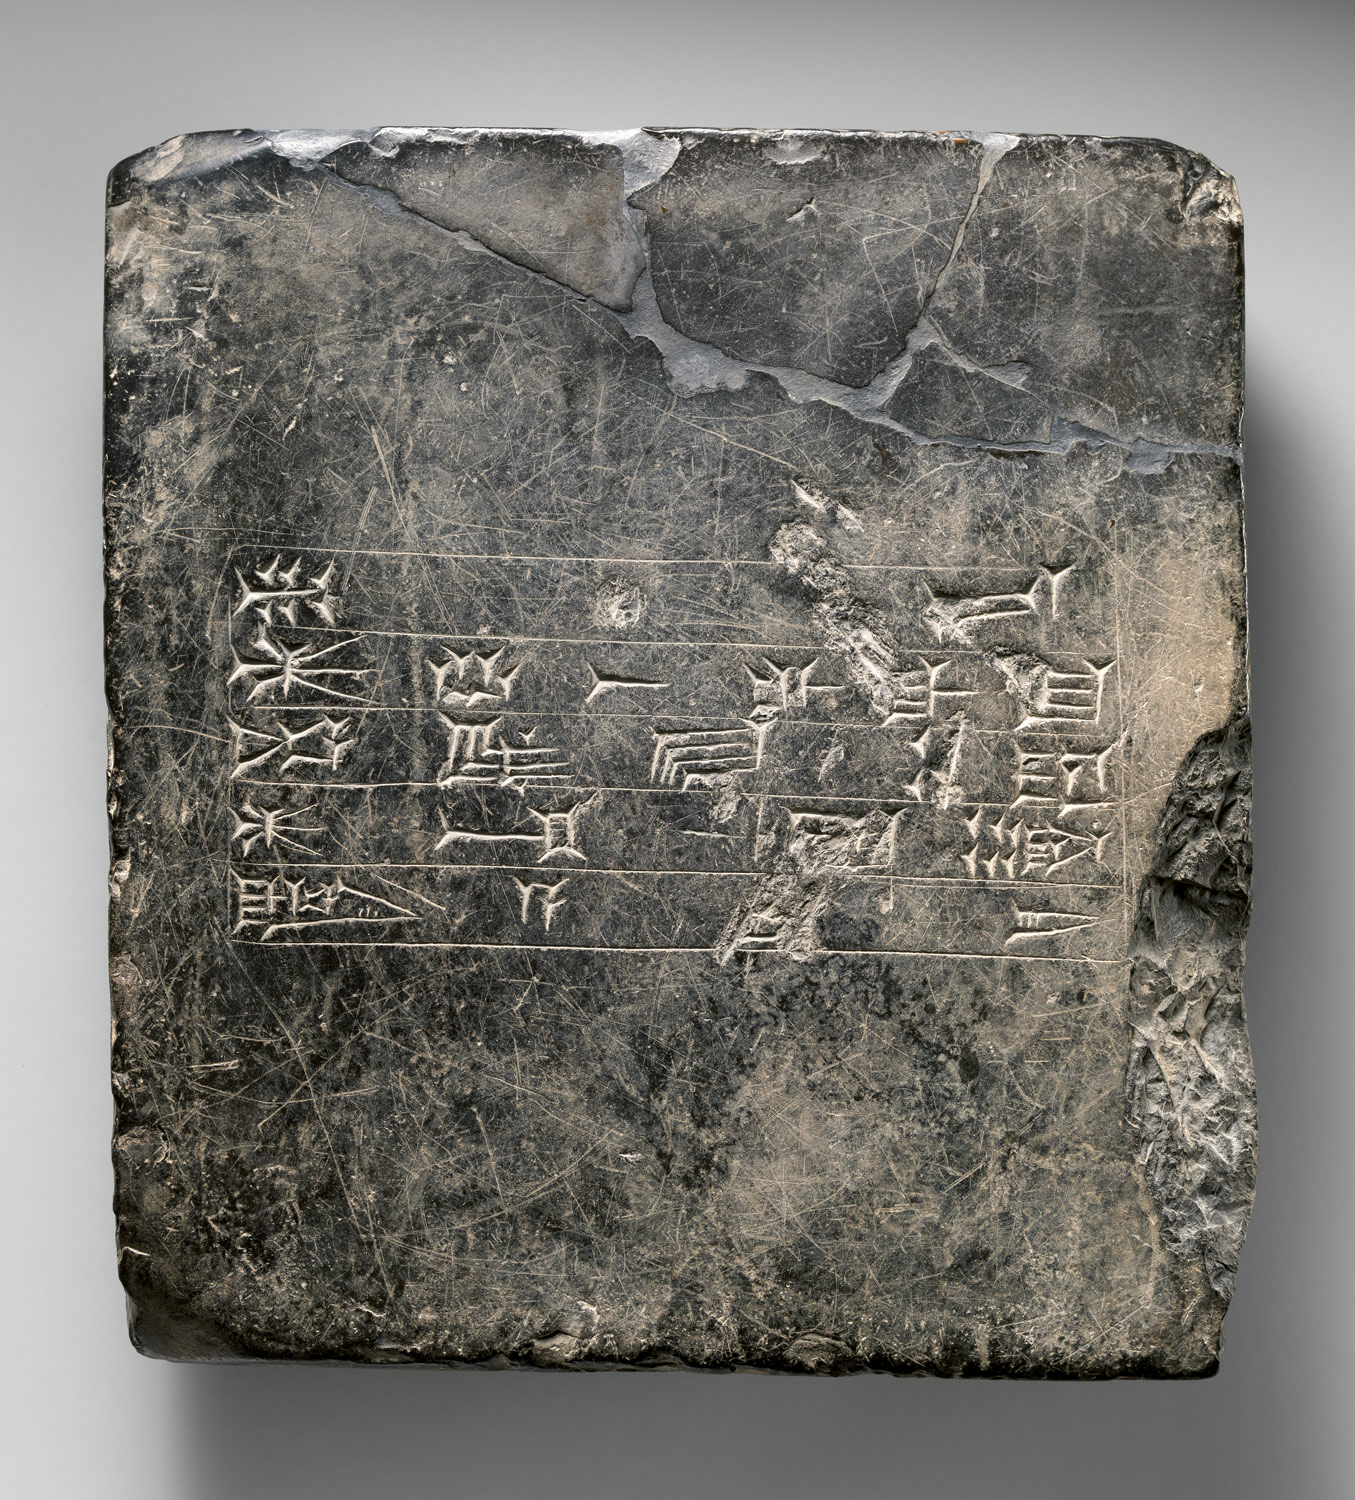
\includegraphics[scale=0.07]{pics/cuneiform.jpg}
    \end{column}
  \end{columns}
  Example:
  \begin{itemize}
    \item Python language
    \item Julia language
    \item R statistical language
  \end{itemize}
\end{frame}


\begin{frame}[label=compiled]
  \frametitle{Writing your own program}
  \framesubtitle{Compiled languages}
  Use a low level \focus{programming language} which is parsed by a program
  called \textit{compiler} to create a system binary program
  \begin{columns}[T]
    \begin{column}{.23\textwidth}
      \includegraphics[scale=0.35]{pics/225px-ISO_C++_Logo.png}
    \end{column}
    \hfill
    \begin{column}{.76\textwidth}
      \begin{itemize}
        \item \textbf{Pros} : Fast execution time, tailored processing to the
          problem to solve
        \item \textbf{Cons} : Need to learn a programming language, not as
          flexible as a scripting language, may require writing code even
          for very simple and common tasks best approached by generic 
          system programs.
      \end{itemize}
    \end{column}
  \end{columns}
  Example:
  \begin{itemize}
    \item Fortran Programming Language
    \item C/C++ Programming Language
  \end{itemize}
\end{frame}


\begin{frame}[label=whichone]
  \frametitle{Writing your own program}
  \framesubtitle{Which language is THE best}
  There is no a \focus{win all} language.
  \begin{itemize}
    \item Do not use a sledgehammer to crack walnuts
    \item Select the language keeping in mind the problem to solve
    \item Always start from the simplest solution
    \item Invest in learning a new tool only if needed
    \item Consider the problem at hand and split it in simple tasks
    \item Use the best possible tool for each task
    \item Identify performance bottlenecks and solve those
  \end{itemize}
\end{frame}


\begin{frame}[label=Fortran, fragile=singleslide]
  \frametitle{Fortran Language}
  \framesubtitle{Programming like in the 1950}
  \begin{columns}[T]
    \begin{column}{.23\textwidth}
      \vspace{30pt}
      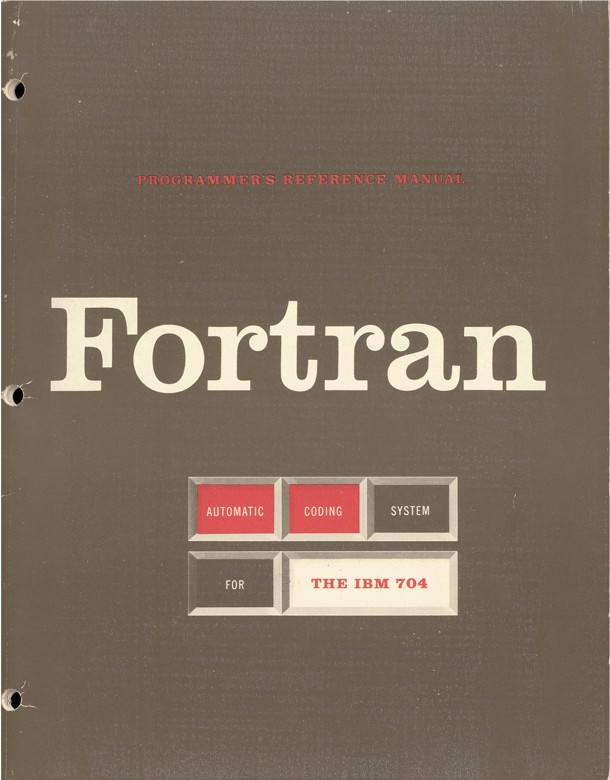
\includegraphics[scale=0.15]{pics/Fortran_acs_cover.jpeg}
    \end{column}
    \hfill
    \begin{column}{.76\textwidth}
      \begin{itemize}
        \item Fortran programs are witten as source text files: \\
          \footnotesize{
            \begin{verbatim}
program count
  integer :: i
  do i = 1, 10
    print *, i
  end do
end program count
            \end{verbatim}
          }
        \item \normalsize{A \focus{compiler program} parses source files and
            create binary object files:} \\
          \footnotesize{
          \code{gfortran -o myprog myprog.f90}
          }
        \item \normalsize{Objects are linked with other objects or
           libraries to create executables:} \\
          \footnotesize{
            \begin{verbatim}
0000000 457f 464c 0102 0001 0000 0000 0000 0000
0000010 0003 003e 0001 0000 06f0 0000 0000 0000
0000020 0040 0000 0000 0000 1a78 0000 0000 0000
0000030 0000 0000 0040 0038 0009 0040 001d 001c
0000040 0006 0000 0004 0000 0040 0000 0000 0000
            \end{verbatim}
          }
      \end{itemize}
    \end{column}
  \end{columns}
\end{frame}


\begin{frame}[label=exercise1, fragile=singleslide]
  \frametitle{Exercise}
  \framesubtitle{Write and compile Fortran 'Hello World'}
  \begin{itemize}
    \item Create a text file \code{hello.f90} with the below content:
      \footnotesize{
      \begin{verbatim}
program hello
  implicit none
  integer , parameter :: stdout = 6
  character(len=*), parameter :: message = 'Helo World'
  character(len=1), parameter :: mark = '!'
  write(stdout,'(a,a)') message, mark
end program hello
      \end{verbatim}
      }
    \item Compile the program into an executable file: \\
      \code{gfortran -o hello hello.f90}
    \item Execute the executable file created: \\
      \code{./hello}
  \end{itemize}
    \begin{alertblock}{Have you noticed?}
      No error is allowed in the code: Fortran Language has very
        strict syntax. But you can misspell the message! \\
      Why we had to run the program with \code{./hello}?
    \end{alertblock}
\end{frame}


\begin{frame}
  \begin{center}
    \frametitle{File Permissions}
    \framesubtitle{How to check file permissions}

    \sidebyside{0.44}{
      \centering
      See permissions: \code{ls -l}
    }{\hfill}{0.52}{
      \begin{center}
        \includegraphics[width=1.00\textwidth]{pics/ls-l.png}
      \end{center}
    }
    \begin{alertblock}{Check this}
      What do you see running \code{ls -l} in the directory where you
        have compiled the \code{hello} program and code? \\
      Can you spot the executable files looking at the permission bits? \\
      Try running \code{ls -al}. Can you tell which are the directories
        from the permission bits?
    \end{alertblock}

  \end{center}
\end{frame}

\begin{frame}[label=executables]
  \frametitle{Executable files}
  \framesubtitle{System programs and user programs}
  \begin{itemize}
    \item An executable file is a file with execute permission bit on
    \item The system programs (\code{ls}, \code{mkdir}, \code{cd},
      \code{gfortran}, etc.) are files with execute permission bit set
      that are stored in predefined directories (\code{/bin}, \code{/usr/bin},
      \code{/usr/local/bin}) that are in the system \code{PATH} for
      searching programs
    \item User executable are not in the \code{PATH} and to run them the
      path to reach the executable, absolute or relative, must be provided
    \item \code{PATH} is an environment variable. More on those next days.
  \end{itemize}
  \begin{alertblock}{Check the system programs}
      Try searching the program \code{ls}. \\
      \code{ls -l /bin/ls} \\
      Where is \code{cd}? And \code{gfortran}?
   \end{alertblock}
\end{frame}


\begin{frame}[label=compiler]
  \frametitle{Compiler flags}
  \framesubtitle{Optional arguments for Fortran programming}
  The compiler is a program and accepts command line arguments. Above we
    have used the \code{-o} option to specify the name of the output.
  \begin{block}{Useful gfortran options}
    \begin{itemize}
        \item \code{-o program} output program name (default a.out)
      \item \code{-Ofast} Optimize program for fast execution time
      \item \code{-O0} Remove all optimization (for debugging)
      \item \code{-g} include debugging information
      \item \code{-Wall} Enables commonly used warning options pertaining to
          usage recommend avoiding and that are easy to avoid
      \item \code{-pedantic} check program for Fortran standard conformance
      \item \code{-fcheck=all} perform all available run-time checks
      \item \code{-fbacktrace} print the whole trace of the error
  \end{itemize}
  \end{block}
\end{frame}


\begin{frame}[label=exercise2, fragile=singleslide]
  \frametitle{Exercise}
  \framesubtitle{Debug a Fortran program}
  \begin{itemize}
    \item Create a text file \code{error.f90} with the below content:
      \footnotesize{
      \begin{verbatim}
program error
  implicit none
  integer, parameter :: im = 2
  integer, dimension(im,im) :: matrix
  integer :: j
  do j = 1 , 2*im
    do i = 1 , 2*im
      matrix(i,j) = i*j
      print*, matrix(i,j)
    end do
  end do
end program error
      \end{verbatim}
      }
    \item Compile and correct the error
    \item Run the program and check the runtime error
    \item Compile in debug:
        \code{-O0 -g -Wall -pedantic -fcheck=all -fbacktrace}
    \item Run the program, check the error and correct the program
    \item Recompile an optimized executable
  \end{itemize}
\end{frame}


\begin{frame}[label=permission]
  \frametitle{File permissions}
  \framesubtitle{RWX bits}
  \begin{columns}[T]
    \begin{column}{.11\textwidth}
      \includegraphics[scale=0.15]{pics/Timbro.jpg}
    \end{column}
    \hfill
    \begin{column}{.89\textwidth}
      \small{
      There are three basic attributes for plain file permissions:
      \begin{itemize}
        \item read \code{r}
        \item write \code{w}
        \item execute \code{x}
      \end{itemize}
      They mean what you would expect. There are three classes of users:
      \begin{itemize}
        \item owner \code{u}
        \item group \code{g}
        \item other \code{o}
      \end{itemize}
      For each of the three classes you have three possible attributes
      to set. \\
      \vspace{10pt}
      For directories:
      \begin{itemize}
         \item read : you can list the content
         \item write : you can create/remove files inside
         \item execute : you can access it and its content
      \end{itemize}
    }
    \end{column}
  \end{columns}
\end{frame}


\begin{frame}
  \frametitle{File Permissions}
  \framesubtitle{Changing file permissions using \code{chmod}}

  \sidebyside{0.42}{
    Change permissions: \code{chmod}

    \code{chmod <who><+/-><what> <file>}

    \begin{itemize}
      \item \code{<who>}:\\
        \code{u} (user),\\
        \code{g} (group),\\
        \code{o} (other),\\
        \code{a} (everybody)
      \item \code{<+/->}: \code{+} to add, \code{-} to remove
      \item \code{what}: \code{r,w,x} as above
    \end{itemize}
  }{\hfill}{0.48}{
  \begin{center}
    \includegraphics[scale=0.23]{pics/chmod.png}
  \end{center}
  }
\end{frame}


\begin{frame}[label=exercise3, fragile=singleslide]
  \frametitle{Scripts and programs}
  \framesubtitle{Creating a shell script executable}

  Let us create an 'hello world' program in shell and execute it.
  \begin{exampleblock}{Shell script}
      Edit a text file \code{hello.sh} and write inside the following:
\begin{verbatim}
#!/bin/bash
echo Hello world
\end{verbatim}
  \end{exampleblock}

  \begin{alertblock}{}
    Can you directly execute the script as we have done with \code{hello}? \\
    Try \code{./hello.sh}
  \end{alertblock}

  \begin{exampleblock}{Use \code{chmod}}
      \code{chmod u+x hello.sh}
  \end{exampleblock}

  \begin{alertblock}{}
    Can you now execute the script?
  \end{alertblock}
\end{frame}


\begin{frame}[label=scriptnotes]
  \frametitle{Notes on the script}
  \framesubtitle{Missing bits}
  \begin{block}{sha-banging magic number}
    The control sequence \code{\#!} at the script start is a so called
      hash bang, or shabang or shebang. The purpose is to act as a magic
      sequence. The program name that follows is the program that must
      be called to execute what is following. \\
      \code{\#!/bin/bash} \\
      \code{\#!/usr/bin/env python3} \\
      \code{\#!/usr/bin/perl}
  \end{block}
  \begin{block}{echo}
    The program \code{echo} is \code{/bin/echo} and it is used to display
      on the screen any provided line following the program name. \\
    Look at the man page for it options.
  \end{block}
\end{frame}


\begin{frame}
  \frametitle{Python language}
  \framesubtitle{Running the python interpreter}
  Python is an interpreted language. Any line of code goes through the
    interpreter in a \focus{Read-Eval-Print Loop} or \focus{REPL}.
  \begin{block}{Install the interpreter}
    \code{ictp-install python3 ipython3 python3-ipython} \\
    \code{ictp-install python3-numpy python3-matplotlib}
  \end{block}
  \begin{block}{Start the interpreter}
    \code{ipython3}
  \end{block}
  \begin{block}{Test the interpreter}
    \code{64*2}
  \end{block}
\end{frame}


\begin{frame}[fragile=singleslide]
  \frametitle{Python language}
  \framesubtitle{Quick and dirty csv plotting}
  \begin{block}{Start the interpreter}
    \code{ipython3}
  \end{block}
  \begin{exampleblock}{ }
    Copy line by line the following:
    \small{
    \begin{verbatim}
from datetime import datetime
import numpy as np
import matplotlib.pyplot as plt

my_data = np.genfromtxt('first.csv',delimiter=',',dtype=None)
precip = np.fromiter((x[3] for x in my_data),float)
dt = list(datetime(x[0],x[1],x[2]) for x in my_data)
timeaxis = np.array(list(np.datetime64(x) for x in dt))
plt.plot(timeaxis,precip)
plt.gcf().autofmt_xdate()
plt.show( )
    \end{verbatim}
    }
  \end{exampleblock}
\end{frame}

\begin{frame}[fragile=singleslide]
  \frametitle{Python language}
  \framesubtitle{From interactive to program}
  \begin{exampleblock}{}
    Write the following in the file \code{plot.py}
    \small{
    \begin{verbatim}
#!/usr/bin/env python3
from datetime import datetime
import numpy as np
import matplotlib.pyplot as plt
my_data = np.genfromtxt('first.csv',delimiter=',',dtype=None)
precip = np.fromiter((x[3] for x in my_data),float)
dt = list(datetime(x[0],x[1],x[2]) for x in my_data)
timeaxis = np.array(list(np.datetime64(x) for x in dt))
plt.plot(timeaxis,precip)
plt.gcf().autofmt_xdate()
plt.show( )
    \end{verbatim}
    }
  \end{exampleblock}

  \begin{alertblock}{What is missing?}
    There is still one passage missing to be able to run the program as
      \code{./plot.py}. Can you tell me what is missing?
  \end{alertblock}
\end{frame}

\end{document}

%vim: tabstop=8 expandtab shiftwidth=2 softtabstop=2 spell spelllang=en_uk
